\section{Introduction}
The prevalence of positioning devices has drastically boosted the scale of trajectory data collection. 
Instances include telemetry chips for animal herding histories, 
GPS devices for urban transportation and wearable devices for personal moving activities. 
These positional data are timestamped and can be viewed as trajectories. 
Data analysis on large-scale trajectories benefits a wide range of applications and services, including traffic planning~\cite{zheng2011urban}, animal analysis~\cite{li2010miningperiodic}, and social recommendations~\cite{bao2013survey}, just to name a few.% CITATIONS FOR THE ABOVE APPLICATIONS.

An important task of data analysis on trajectories is to discover co-moving objects. 
As its name suggests, a \emph{co-movement} pattern~\cite{li2013managing} consists 
of a group of objects that travel together for some duration, where the group is formed
by certain clustering methods. A pattern is prominent 
if the size of the group exceeds $M$ and the length of the duration exceeds $K$, where $M$ and $K$
are user specified parameters. Depends on further constraints on object clustering
and time duration, several specific patterns are proposed in the literature. 

Specifically, on the aspect of object clustering, \emph{flock}~\cite{gudmundsson2006flock} and \emph{group}~\cite{wang2006grouppattern} patterns require objects to be within a disk region.
In contrast, \emph{convoy}~\cite{jeung2008convoy}, \emph{swarm}~\cite{li2010swarm} and
\emph{platoon}~\cite{li2015platoon} patterns require objects to be densely connected. 
In terms of the constraints on time duration, \emph{flock}~\cite{gudmundsson2006flock} and \emph{convoy}~\cite{jeung2008convoy}
require the timestamps to be consecutive. \emph{Swarm}~\cite{li2010swarm}, on the
other hand, do not impose any restrictions. \emph{Group}~\cite{wang2006grouppattern} 
and \emph{platoon}~\cite{li2015platoon} introduce the parameter $L$ to control the minimum length of the local-consecutive
timestamps. 
The compare and contrast of these co-movement patterns are presented in Table~\ref{tbl:existing_co_patterns}.

%Specifically, a \emph{flock}~\cite{gudmundsson2006flock} requires the group to be within a disk region of
%the user specified size.  A \emph{convoy}~\cite{jeung2008convoy} requires a group to be densely connected. Both \emph{flock}
%and \emph{convoy} require a group to appear for at least $k$ consecutive times.  
%\emph{Group}~\cite{wang2006grouppattern} and 
%\emph{Swarm}~\cite{li2010swarm} patterns relax the consecutiveness constraint, where non-consecutive timestamps are allowed in a pattern duration. \emph{Group} pattern require objects in a group to be within a disk region, while \emph{swarm}require the objects in a group to be densely connected.
%Recently,
%\emph{platoon}~\cite{li2015platoon} pattern is proposed to impose a fine-grained control on the consecutiveness of the duration. In \emph{platoon}, the duration of a group needs to have the local-consecutive portion of size no less than the user-specified $L$.

\begin{table}
\centering
\begin{tabular}{|c|c|c|c|}
\hline 
Pattern & Clustering Method & Consecutiveness on Duration \\ 
\hline 
Flock~\cite{gudmundsson2004flock} & Disk region &  Consecutive \\ 
\hline 
Convoy~\cite{jeung2008convoy} & Density &   Consecutive \\ 
\hline 
Group~\cite{wang2006grouppattern} & Disk region &  Local consecutive $\geq L$ \\ 
\hline 
Swarm~\cite{li2010swarm} & Density  & No constraint \\ 
\hline 
Platoon~\cite{li2015platoon} & Density &  Local consecutive $\geq L$ \\ 
\hline 
\end{tabular} 
\caption{Existing Co-movement Patterns}
\label{tbl:existing_co_patterns}
\end{table}

%of densely connected objects that travel together for at least $k$ consecutive time. A \emph{swarm}~\cite{li2010swarm} relax the consecutiveness of \emph{convoy}.
% 
%To formally define the pattern, the temporal dimension of trajectories is descritized into snapshots, where each snapshot contains the geographical information of all moving objects. 
%Given a member size constraint $n$, a temporal constraint $k$, a \emph{co-movement} pattern finds a cluster of objects with at least size $n$ and close in spatial proximity for at least $k$ snapshots. 
%Recently, there have been several works extending the basic pattern to incorporate more advanced temporal constraints. For instance, Jeung et al. proposed \emph{convoy} pattern, which requires the snapshots to be consecutive; Li et al. proposed \emph{swarm} pattern, which relaxes the consecutiveness of snapshots and Li et al. proposed \emph{platoon} pattern which imposed a \emph{minimum local length} on the snapshots. 
%PLEASE BE MORE SPECIFIC FOR THE THREE PATTERNS. ALSO, ADD THE CITATIONS.


%We first provide a synthetic example to better illustrate these patterns in Figure~\ref{fig:related_work}, and the formal definitions are described in Section~\ref{sec:definition}.
We illustrate these co-movement patterns in Figure~\ref{fig:related_work} with an example of five trajectories.
First, the temporal domain is discretized into five snapshots. 
In each snapshot, the objects are clustered as shown in the dotted circle.
By setting the parameters $M=2, K=3$, we are able to discover \emph{convoy}, \emph{flock}, and \emph{swarm} patterns. 
It is notable that \emph{convoy} and \emph{flock} have the same result pattern, this is because both patterns share 
the same constraints on the time duration. 
\emph{Swarm} pattern results in a super set of \emph{convoy} and \emph{flock} patterns, as it 
does not require any consecutiveness on the time duration. By setting $L=2$, we find three \emph{group} patterns. 
If further set $M=2,K=3$, two \emph{platoon} patterns are found. It is observable that the pattern $\langle\{O_5,O_6\}\{1,4,5\} \rangle$ is a \emph{swarm} but is neither a \emph{platoon} nor a \emph{group} since one of its local consecutive duration (i.e. $\{1\}$) is less than $2$. However, $\langle\{O_5,O_6\}\{1,4,5\} \rangle$ can be reduced to $\langle\{O_5,O_6\}\{4,5\} \rangle$ which is a \emph{group} pattern because \emph{group} pattern only restricts the local consecutiveness but not the total size of a duration. 

% we achieve two \emph{platoon} patterns.
% 
%By setting $M=2$, the spatial clusters with at least $2$ objects are displayed with the same shape. Since \emph{Convoy} pattern requires the set of objects to be clustered for $k$ \emph{consecutive} snapshots, there results in only one such pattern ($\{o_3,o_4\}\{t_1,t_2,t_3\}$) when $k$ is set to $3$. \emph{Swarm} pattern relaxes the consecutiveness of duration, thus there are three patterns discovered. \emph{Platoon} pattern requires that each local consecutive duration needs to have at least certain length, which is indicated by an additional parameter $l$. When $l$ equals 2, there are two patterns discovered. Note that $\{o_6,o_7\}\{t_1,t_4,t_5\}$ is not included in the platoon pattern since $t_1$ is the local consecutive snapshot with duration 1, which is less than $l$. CAN WE SUPPORT THE GROUP AND FLOCK PATTERN? IF YES, WHY NOT PUT THEM IN THE FIGURE?
%
%FOR THE FIGURE: 1) ENLARGE THE FONT SIZE IN THE FIGURE 2) WHY THERE IS NO $o_5$. 3) WHY OBJECTS IN DIFFERENT COLORS AND SHAPES ARE NOT CLEAR. YOU CAN REMOVE COLOR. 4) PUT THE OBJECTS BELONGING TO THE SAME CLUSTER IN THE SAME LINE.

\begin{figure} [h]
\center
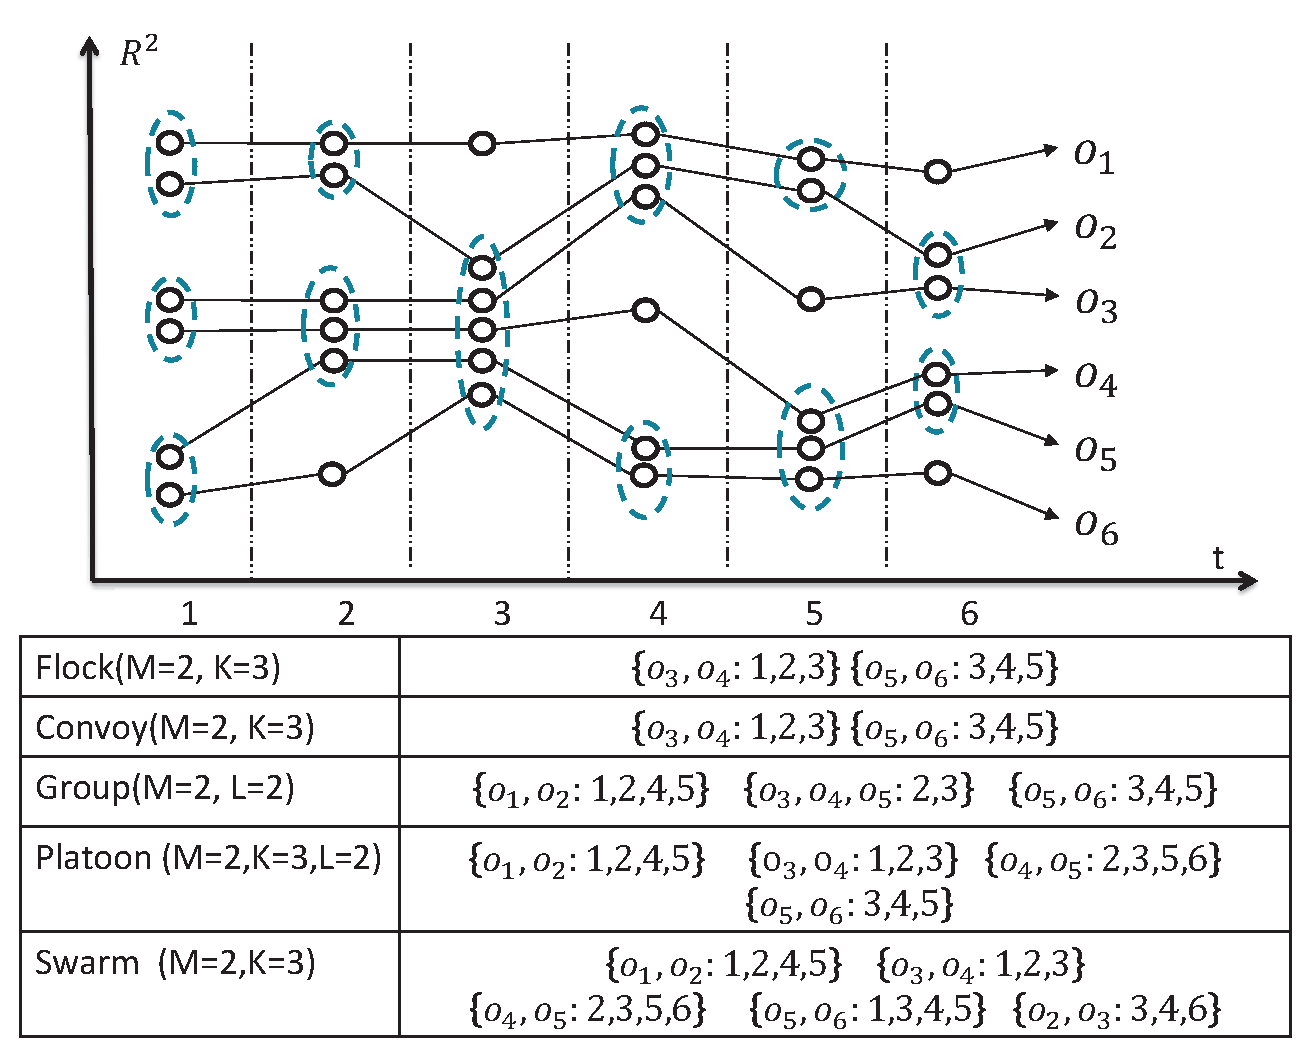
\includegraphics[width=0.5\textwidth]{related_work.eps}
\caption{Trajectories and Co-Movement Patterns}
\label{fig:related_work}
\end{figure}

%We notice that, \emph{platoon} pattern is more general than \emph{convoy} and \emph{swarm}. This is because by setting appropriate $l$, \emph{platoon} can be reduced to \emph{convoy} and \emph{swarm} respectively~\cite{li2015platoon}. However, we observe that \emph{platoon} pattern is to loose on the temporal domain thus may result in less significant patterns. For example in Figure~\ref{fig:platoon_weakpoint}.


%
%\begin{figure}[h]
%\center
%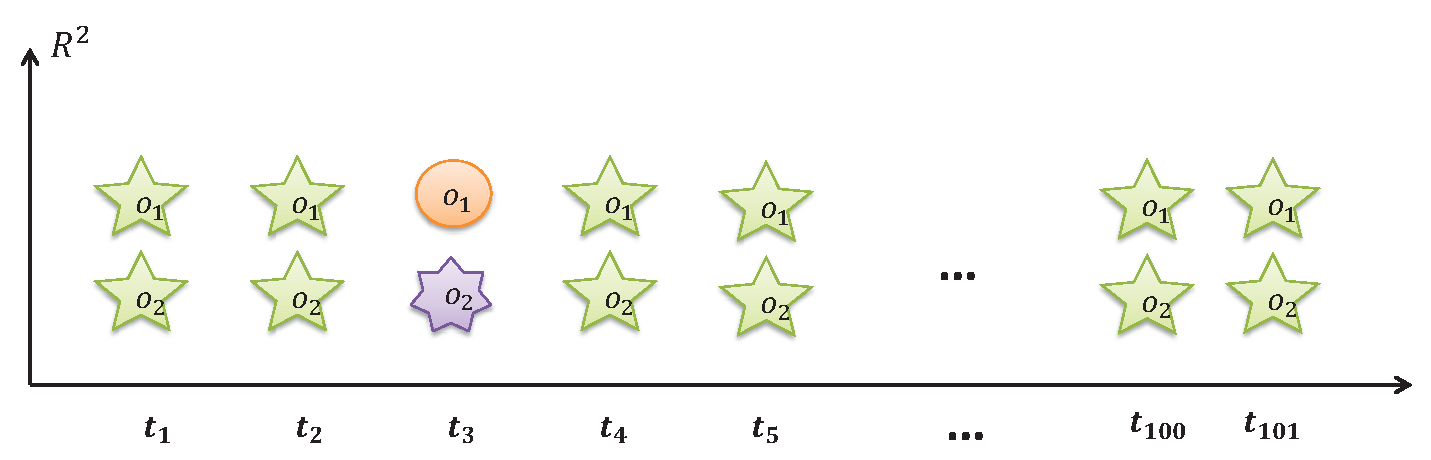
\includegraphics[width=0.5\textwidth]{platoon_weakpoint.eps}
%\caption{Miss-pattern in platoon}
%\label{fig:platoon_weakpoint}
%\end{figure}

%In platoon, a pattern for $n=2,k=4,l=2$ could be $\{o_1, o_2\}\{t_1,t_2,t_4,t_5,t_{100},t_{101}\}$. However, the snapshots $t_{100}$ and $t_{101}$ is too far away from previous snapshots. Such two snapshots are in less relation with previous snapshots and thus should be removed from the pattern. Based on this observation, we defined a \emph{generalized co-moving} pattern (as in Section~\ref{sec:definition}) to provide a more fine granular control of the pattern. In \emph{generalized co-moving} pattern, a parameter $g$ is introduce the control the \emph{maximum gap} allowed between consecutive snapshots. By so doing our generalized co-moving pattern is more expressive and can represent all the existing co-moving patterns.

%In step with the advances in localization technologies, the growth in the volume of trajectory data is rapid. Traditional single-machine methods face severe scalability problem in handling large trajectory data. For example, as reported in~\cite{li2015platoon}, a \emph{Swarm} pattern takes around 100 seconds to discover for 100k trajectories. With upto billions of trajectories in nowadays datasets, such approaches apparently become unfeasible. To tackle this challenge, we propose a  paralleled solution for discovering \emph{generalized co-moving} patterns. We then deploy our idea on the modern MapReduce platform. As our experiments show, our solution achieves well load-balance and can process billions of trajectories in XXX seconds. Several optimizations are also designed to boost our solution to be orders of magnitudes faster than baseline algorithms.

%In practice, it is cumbersome to design tailed solutions to different types of co-movement pattern discovery. 

%In reality, it is cumbersome to design tailed solutions to support 
%generality and scalability

%In this paper, our primary objectives are solving two 

As can be seen, there are various co-movement patterns requested by different applications and it is cumbersome to design a tailored solution for each type. Hence, there is an urgent demand for a general platform to support all these co-movement patterns. Another issue with existing methods is that they are built on top of centralized indexes that are not scalable. The maximum number of trajectories ever evaluated is up to hundreds of thousands of trajectories. In practice, it is rather common to collect millions of trajectories. We, for the first time, evaluate the pattern mining performance at the million scale and report the performance in Figure~\ref{}. The results show that their performance degrades dramatically as the dataset size scales up. None of them can handle millions of trajectories efficiently. 

Therefore, our primary contributions in this paper are to close these two gaps. First, we propose a general co-movement pattern definition to incorporate all the related variants in the existing literature. We observe that even though \emph{platoon} is the most general pattern among existing patterns, it suffers from \emph{loose connection} problem. This is because that \emph{platoon} allows the timestamps in a pattern duration to be in arbitrary distance, making the object group loosely
connected. For instance, patterns with duration $\{1,2,100,101\}$ could be a valid \emph{platoon}; however, the two timestamps $2,100$ are too far from each other. Such a pattern is likely to be induced by periodic movements of unrelated objects thus is of low interests. To cope with this anomaly, we propose the \emph{general co-movement pattern} by introducing the gap parameter $G$, which requires the distance of timestamps in the duration to be no larger than $G$. By so doing, we gain a fine-grained control over the pattern duration, which alleviates the \emph{loose connection} problem. Meanwhile, the general co-movement pattern does not concede its expressiveness. As we show in later sections, the general co-movement pattern is able to reduce to existing patterns by setting appropriate parameters.

 
Second, we propose a parallel solution based on Spark for scalable pattern mining. Our
solution is a three-step MapReduce alike approach. First, trajectories are partitioned
into snapshots where clusters from each snapshots are formed in parallel. Second, 
clusters at various timestamps are shuffled and regrouped. Third, the general co-movement patterns
are mined from each group. The challenge here is to ensure that
the patterns mined at step three is complete. If not, further shuffles and computations are required which 
significantly drag down the system performance. In order to resolve the challenges and meanwhile keep the 
shuffle amount at each stage to a minimum, 
we design a novel star-based partition scheme to efficiently partition objects based on their
belonging clusters. Based on the star partition, we then propose a series of optimization techniques which
largely improve the system performance.

Third, we conduct a set of extensive experiments on XXX datasets with million-scale trajectories. The results show that XXX.

The rest of our paper is organized as follows: Section~\ref{sec:related_works} summarizes the relevant literature on 
trajectory pattern mining; Section~\ref{sec:definition} forms the definition of the general co-movement pattern mining; Section~\ref{sec:system_overview} presents our parallel architecture; The solution of mining the general co-movement pattern mining is presented in Section~\ref{sec:solution} and Section~\ref{sec:optimization} discuss various optimization techniques to boost the system performance; Section~\ref{sec:experiment} conducts extensive experiments to showcase the usefulness and efficiency of our system and finally Section~\ref{sec:conclusion} concludes our paper.

